% Full chain: pdflatex -> bibtex -> pdflatex -> pdflatex
\documentclass[11pt,en]{elegantpaper}

\title{Ensembling learning applied to ACLR:\\ Artificial Characters Learning Problem}
\author{Wangzhihui Mei 2019124044 6603385}
\institute{CCNU-UOW JI}

% \version{0.09}
\date{}

% cmd for this doc
\usepackage{array}
\newcommand{\ccr}[1]{\makecell{{\color{#1}\rule{1cm}{1cm}}}}

\begin{document}

\maketitle

% \begin{abstract}
% This documentation illustrates the usage of the \href{https://github.com/ElegantLaTeX/ElegantPaper}{ElegantPaper} template. This template is based on the standard \LaTeX{} article class, which is designed for working paper writing. With this template, you can get rid of all the worries about the format and merely focus on writing. For any question, please leave a message on \href{https://github.com/ElegantLaTeX/ElegantPaper/issues}{GitHub::ElegantPaper/issues}. Want to know more about Elegant\LaTeX{} Templates? Please visit: \href{https://github.com/ElegantLaTeX}{https://github.com/ElegantLaTeX}.\par
% \keywords{Elegant\LaTeX{}, Working Paper, Template}
% \end{abstract}


\section{Introduction}
This database has been artificially generated by using a first order theory which describes the structure of ten capital letters of the English alphabet and a random choice theorem prover which accounts for etherogeneity in the instances. The capital letters represented are the following: A, C, D, E, F, G, H, L, P, R. Each instance is structured and is described by a set of segments (lines) which resemble the way an automatic program would segment an image. 

Each instance is stored in a separate file whose format is the following:
\begin{lstlisting}
CLASS OBJNUM TYPE XX1 YY1 XX2 YY2 SIZE   DIAG
1     0      line 0   0   0   13  13.00  45.28
1     1      line 20  0   22  15  15.13  45.28
1     2      line 0   13  22  15  22.09  45.28
1     3      line 0   13  0   27  14.00  45.28
1     4      line 22  15  23  39  24.02  45.28
1     5      line 0   27  23  39  25.94  45.28
\end{lstlisting}

\begin{figure}[h]
	\centering
	
\includegraphics[width=0.5\textwidth]{image/chars}
	\caption{The generated characters}
	\label{chars}
\end{figure}

where CLASS is an integer number indicating the class as described below, OBJNUM is an integer identifier of a segment (starting from 0) in the instance and the remaining columns represent attribute values. \cite{schapire1999improved}.

The generated character image is like Figure \ref{chars}


\section{Model construction and parameter optimization}
\subsection{Data pre-process}
The character described by segments is represented as the vertex pair, we transform them to binary grid ($12\times 8$), like Figure \ref{transform}.

\begin{figure}[h]
	\centering
	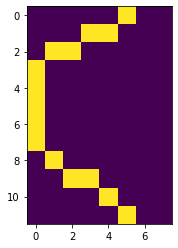
\includegraphics[width=0.3\textwidth]{image/C_array}
	\caption{The representation of "C"}
	\label{transform}
\end{figure}

Then the problem is transformed into one like the MNIST classification problem. The feature is the flattened 0-1 pixel, whose dimension is $96\times 1$, the label is "A", "C", "D", "E", "F", 
"G", "H", "L", "P", "R", which correspond to the numbers 0 through 9. 


We got 6000 training data from the primitive dataset. We shuffled them and use 70\% of the data as training data, 30\% as test data. The label distribution of training data is like Figure \ref{dist_y}
\begin{figure}[h]
	\centering
	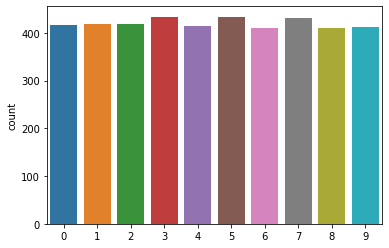
\includegraphics[width=0.4\textwidth]{image/dis_y}
	\caption{The label distribution of training data}
	\label{dist_y}
\end{figure}

\subsection{Model construction}
I applied linear models(Linear Regression, SGD, SVM), bayes model, neural network model(MLP), decision tree model, random forest model, extra tree model, and them ensemble them as voting model.
\subsubsection{Logistic Regression Model}
Regarding logistic regression, it can be summarized in one sentence: Logistic regression assumes that the data obey Bernoulli distribution, and uses the gradient likelihood method to solve the parameters through the maximum likelihood function method to achieve the purpose of classifying the data.

Our parameter tuning:
\begin{itemize}
	\item multi\_class: In this case, the pattern only belong to one class, we set it to 'multinomial'
	\item max\_iter: Set the maximum number of iterations taken for the solvers to converge to 1000.
	\item solver: For multiclass problems, only ‘newton-cg’, ‘sag’, ‘saga’ and ‘lbfgs’ handle multinomial loss; ‘liblinear’ is limited to one-versus-rest schemes, we tried and selected 'saga'.
	\item n\_jobs: Set to -1 to use all CPU cores to calculation.
	\item penalty: Set to 'l1' to get better weight sparsity.
\end{itemize}

\subsubsection{SGD}
This model is Linear classifiers with SGD training. Stochastic gradient descent(SGD) uses only one sample at a time to calculate the gradient of the objective function. The formula is:
$$\theta=\theta-\alpha \nabla_{\theta} J\left(\theta ; x^{i}, j^{i}\right)$$
The cost function is:
\begin{equation}
	J{train}(\theta)=\frac{1}{m}\sum{i=1}^{m}\frac{1}{2}(h_{\theta}(x^{(i)})-y^{(i)})^{2} = \frac{1}{m}\sum{i=1}^{m}cost(\theta;x^i,j^i)
\end{equation}
Where $\operatorname{cost}\left(\theta ; x^{i}, j^{i}\right)=\frac{1}{2}\left(h_{\theta}\left(x^{(i)}\right)-y^{(i)}\right)^{2}$

Use the loss function of each sample to derive the partial gradient of $\theta$ to get the corresponding gradient to update $\theta$:
$$\theta_{j} = \theta_{j} + \alpha(y^i - h_{\theta}(x^i))x{j}^{i}$$

Stochastic gradient descent is iteratively updated once by each sample, the calculation is very fast and suitable for updating the model online. However, the problem with SGD is that there is more noise than BGD, so that SGD does not go to the overall optimization direction every iteration, and the search process in the solution space seems blind. 

When using SGD we can choose to start with a learning rate of 1.0 or 0.1. Check it on the verification set at intervals.If the cost does not drop, the learning rate is halved.

Our parameter tuning:
\begin{itemize}
	\item loss: Set to ‘log’ loss to give logistic regression, a probabilistic classifier. 
	\item penalty: Set to 'l2'
	\item n\_job: Set to -1 to use all processors.
	\item learning\_rate: ‘optimal’: $eta = 1.0 / (alpha * (t + t0))$ where $t0$ is chosen by a heuristic proposed by Leon Bottou\cite{bottou2003stochastic}.
\end{itemize}

\subsubsection{SVM}
We applied grid search to find the optimized $C$ and $gamma$. We applied binary search method and  narrow the search iteratively. The we got the optimized $C=4.5$ and $gamma=0.06$, see in Figure \ref{bestsvm}.

\begin{figure}[h]
	\centering
	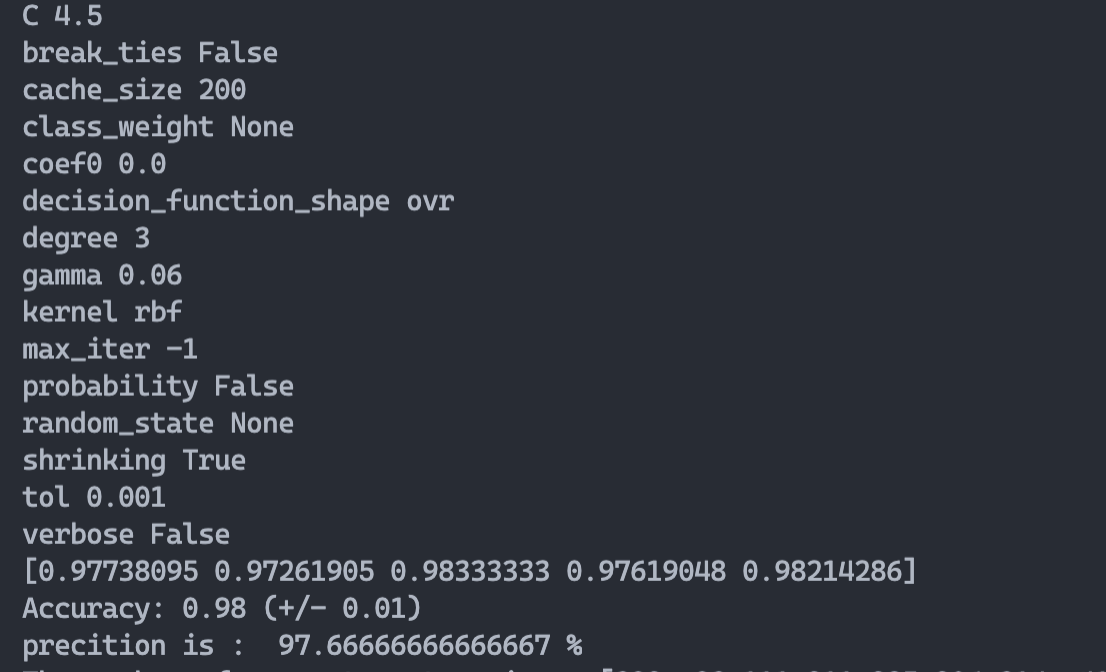
\includegraphics[width=.5\textwidth]{image/bestsvm}
	\caption{Grid search SVM parameters}
	\label{bestsvm}
\end{figure}


My parameter tuning:
\begin{itemize}
	\item C: Regularization parameter. The strength of the regularization is inversely proportional to C. Must be strictly positive. 
	\item kernel: 'rbf'
	\item gamma: 0.06, Kernel coefficient for ‘rbf’, ‘poly’ and ‘sigmoid’.


\end{itemize}


This is the number of support vectors of each class accordingly: [389  90 109 207 285 203 308  44 236 199].
\subsubsection{Decision Tree}
Decision tree is a machine learning method using statistical probability analysis. It represents a kind of mapping between object attributes and object values, and each one in the tree represents a judgment condition indicating an object attribute, which corresponds to an object that meets the condition. The leaves of the tree represent the prediction results of the object.

We use grid search to find the best parameters, see in Figure \ref{bestdt}.
\begin{figure}[h]
	\centering
	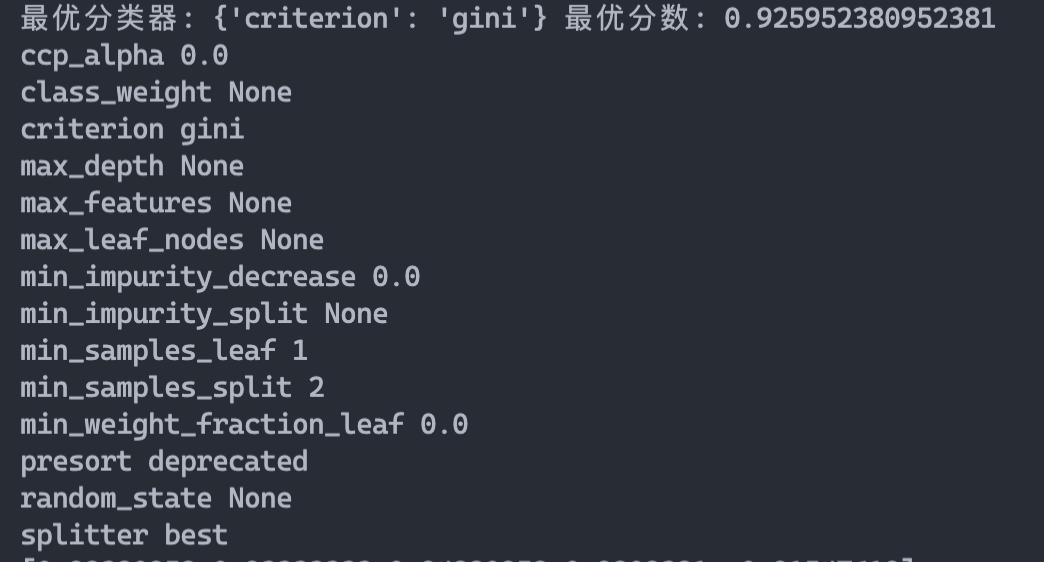
\includegraphics[width=.5\textwidth]{image/bestdt}
	\caption{Grid search decision tree parameters}
	\label{bestdt}
\end{figure}

My parameter tuning:
\begin{itemize}
	\item criterion: 'gini'. Supported criteria are “gini” for the Gini impurity.
	\item min\_samples\_leaf: 1. The minimum number of samples required to be at a leaf node. 
	\item min\_samples\_split: 2. The minimum number of samples required to split an internal node.
\end{itemize}


\section{Evaluation}
An efficient instance selection algorithm to reconstruct training set for support vector machine\cite{liu2017efficient}

\section{Conclusion}
This 


\bibliography{ref}
\end{document}
